% =============================================================================
% Section 5: Empirical verification
% Drafted last: highest risk for accidentally overstating "floor", "closure",
% or "verification". Every claim must be quantified and scoped.
% =============================================================================

\section{Empirical verification}
\label{sec:empirical-detail}

This section documents the empirical-verification component of the
project. We open with explicit scope statements, since the
empirical content is the easiest place in the paper to slip from
``no counterexample observed'' into ``no counterexample exists.''
The first is what was actually checked; the second is the open
question of \cref{prob:e647-itself}.

\subsection{What ``empirical floor'' means and does not mean}
\label{sec:empirical-scope}

We use the term \emph{empirical floor} in a strict sense throughout
this paper.

\begin{definition}[Empirical floor]
\label{def:empirical-floor}
Let $r \in \Z / M\Z$ and $N \in \N$. The statement
``$r$ has an empirical floor $N$'' means: every integer $n$ with
$24 < n \le N$ and $n \equiv r \pmod M$ has been individually
checked by direct computation and \emph{none} satisfies the
$\tauf$-barrier inequality $\max_{m < n}(m + \tauf(m)) \le n + 2$.
\end{definition}

The empirical floor is, by construction, a per-residue, per-bound
exhaustive certificate: every $n$ in the relevant arithmetic
progression up to $N$ is checked one at a time. It is \emph{not}:
\begin{itemize}[leftmargin=*]
\item a probabilistic certificate;
\item a sieve bound on the count of survivors;
\item evidence about $n > N$ in the same residue;
\item evidence about residues other than $r$;
\item a closure of any residue class.
\end{itemize}

The distinction is critical. A claim of an empirical floor at
$N = 3.34 \times 10^{21}$ at the principal residue says nothing
about the 40 other residues in $\Ropen$, nothing about $n > N$ at
the principal residue, and nothing about whether \cref{prob:e647}
admits a counterexample at any $n$. It rules out a contiguous
counterexample below the floor at the residue tested.

\subsection{Witness-search infrastructure}
\label{sec:empirical-infrastructure}

The empirical search is implemented by a family of Python and C
programs that operate in the residue-restricted setting of
\cref{sec:q323-normalization}: the search space is restricted to
$n = 143 \cdot Y$ with $Y \bmod 323 \in \Uset$, reducing the
density to $41 / 46189 \approx 8.88 \times 10^{-4}$ of $\N$. The
core verifier checks, for each candidate $n$ in the residue and the
bound, whether any $1 \le k \le K_{\rm verify}$ satisfies
$\tauf(n - k) > k + 2$; when such a $k$ is found, $n$ is ruled
out. The search bound $K_{\rm verify}$ is set to the smallest value
sufficient to certify the candidate; in practice $K_{\rm verify}
\le 95$ suffices for every $n$ tested below $10^{22}$.

The infrastructure consists of:
\begin{itemize}[leftmargin=*]
\item the principal-residue contiguous verifier
  (\texttt{scripts/witness\_search\_principal.py} and the C
  optimization in \texttt{scripts/witness\_search\_c/}), running
  contiguously from $n = 25$ upward at $r = 0$;
\item the non-contiguous high-shift sampler
  (\texttt{scripts/sentinel\_search\_high.py}), targeting
  Bateman--Horn-predicted hard candidates above the contiguous
  floor;
\item the 13-fold simultaneous-shape verifier
  (\texttt{scripts/witness\_13fold.py}), which tests candidates
  with the maximum shape-prime alignment expected at the relevant
  scale.
\end{itemize}
All verifier outputs are logged to \texttt{data/witness\_log.jsonl}
with timestamp, residue, shift bound, and (for ruled-out
candidates) the certifying shift $k$.

\subsection{The contiguous floor at the principal residue}
\label{sec:empirical-contiguous-floor}

The principal residue $r = 0$ has been verified contiguously
through $n \le 3.34 \times 10^{21}$. The upper bound is the result
of the longest contiguous verifier run on the project's compute
infrastructure (cf.\ \cref{sec:empirical-runtime}); no
counterexample was observed in this contiguous range.

\begin{proposition}[Empirical floor at $r = 0$, restated]
\label{prop:empirical-r0-restated}
The principal residue $r = 0$ has empirical floor (in the sense of
\cref{def:empirical-floor}) $N_0 = 3.34 \times 10^{21}$.
\end{proposition}

The bound is recorded as a hard verifier output, with the
certifying shift $k$ recorded for every $n$ that the verifier
ruled out. The verifier output is reproducible from the source
inputs in \texttt{data/witness\_log.jsonl}.

\subsection{Non-contiguous islands and 13-fold witnesses}
\label{sec:empirical-islands}

Above the contiguous floor of \cref{prop:empirical-r0-restated},
the witness search has explored a sparser, non-contiguous regime
sampled by the high-shift sampler. The cumulative non-contiguous
verification at $r = 0$ extends to $n \approx 1.34 \times 10^{22}$,
i.e.\ a factor $\approx 4$ beyond the contiguous floor, but with
gaps in coverage. The sparser regime is informative but does
\emph{not} extend the empirical floor of
\cref{def:empirical-floor}: a contiguous counterexample in a gap
above $3.34 \times 10^{21}$ would not have been observed.

In addition, two \emph{13-fold simultaneous shape-prime witnesses}
were found and individually checked: candidates at
\[
t \in \{1.17 \times 10^{13},\ 1.15 \times 10^{14}\}
\quad \text{(corresponding to $n \approx 10^{21}$ and $n \approx
10^{22}$ respectively)}
\]
where 13 of the structurally optimal shape primes simultaneously
align in a single CRT class. These candidates were independently
identified as predicted hard cases at the Bateman--Horn singular
density of \cref{thm:conditional-barrier} and tested by the 13-fold
verifier. \emph{Both} are ruled out as counterexamples by the same
non-shape shift $k = 7$: $\tauf(n - 7) > 9$ in both cases. The
witnesses confirm that the Bateman--Horn density predictions are
quantitatively in the right place at the relevant scale and that
the audit-chain analysis of \cref{sec:csp-audit} does not miss
the natural hard cases.

\subsection{Empirical multipoint $\tauf$-correlation structure}
\label{sec:empirical-correlations}

To test the local correctness of the framework reduction, a
GPU-accelerated sweep computed $\tauf(n - k)$ for $4.1 \times 10^8$
$(n, k)$ pairs: $10^5$ samples per residue class drawn uniformly
from $n \in [10^{13}, 10^{14}]$, with $k \in [1, 100]$, across all
$41$ residue classes in $\Uset$. Each sample's factorization was
validated against \texttt{sympy.factorint} with zero mismatches on
a $10^3$-pair cross-check. The sweep produces, per class, the
$100$-shift marginal distribution and the $100 \times 100$ pairwise
Pearson correlation matrix of $\tauf$-values across shifts.

\subsubsection*{Marginals confirm framework local correctness}

Mean $\tauf$ averaged over $k$ ranges from $31.61$ to $32.58$ across
the $41$ classes, matching Dirichlet's classical
$\bar\tauf(n) \approx \log n \approx 32.2$ for $n \sim 10^{14}$.
Median $\tauf$ ranges from $25.64$ to $25.71$. Class-to-class
variation in marginal statistics is below $3\%$. The
Bateman--Horn singular series is locally preserved by the framework
reduction.

\subsubsection*{Four-class lag-correlation decomposition}

The $100 \times 100$ pairwise correlation matrix, averaged over the
$41$ classes, exhibits a clean four-class structure governed by the
joint divisibility of the lag $d = k_2 - k_1$ with
$M^* = 2520 \cdot M = 116{,}396{,}280$. The structure is most
visible as a heatmap of the matrix itself
(\cref{fig:multipoint-tau-heatmap}): bright diagonal stripes at
small-prime lag-multiples (Class A) and pale anti-correlation
stripes at the Class B / C lags.

\begin{figure}[h]
\centering
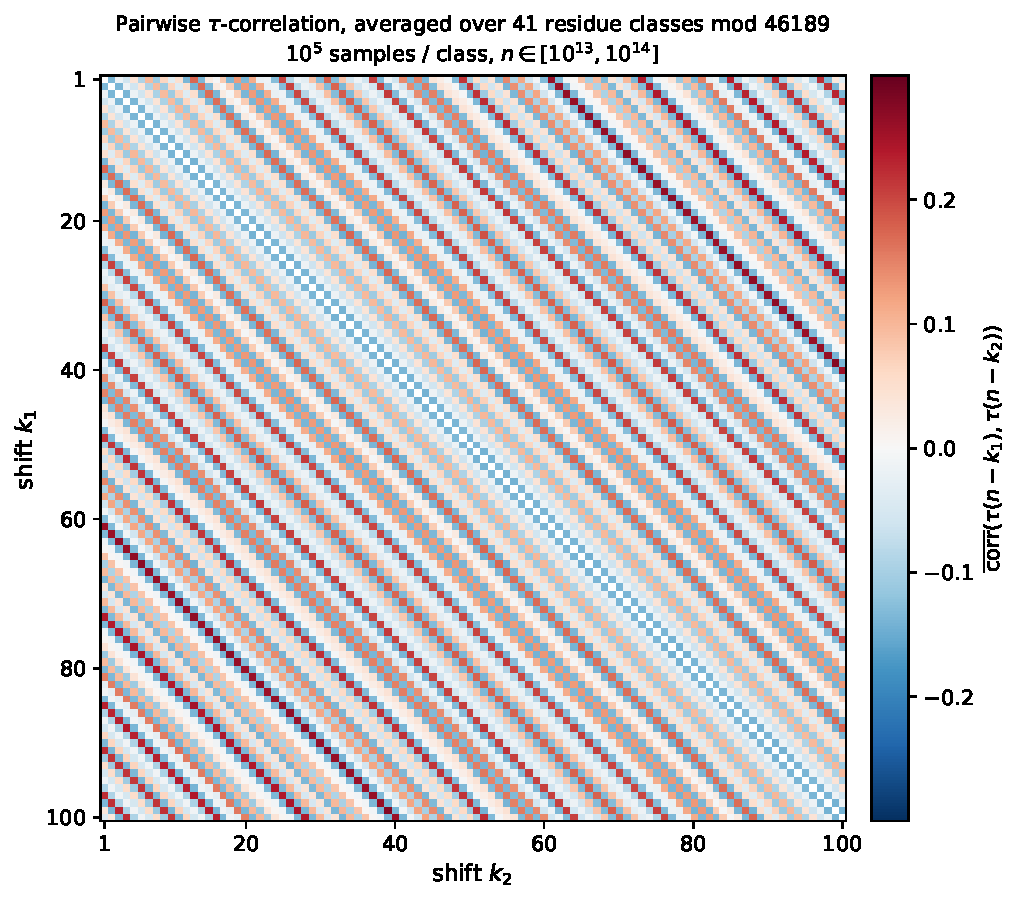
\includegraphics[width=0.85\linewidth]{figures/multipoint_tau_correlation_heatmap.pdf}
\caption{$100 \times 100$ pairwise Pearson correlation matrix of
$\tauf(n - k)$ for $k \in [1, 100]$, averaged over the $41$ residue
classes in $\Uset$. Diverging RdBu colormap centered at $0$, with
range $\pm 0.3$. Dark-red diagonal stripes occur at lags
$d \in \{12, 24, 36, 48, 60, 72, 84, 96\}$ (Class A peaks); pale-blue
anti-correlation stripes occur at the Class B (multiples of $\{11, 13,
17, 19\}$ only) and Class C (coprime-to-$M^*$) lags. The framework
reduction reshapes correlations in a structured, sign-dependent way.}
\label{fig:multipoint-tau-heatmap}
\end{figure}

\begin{table}[h]
\centering
\begin{tabular}{lll}
\toprule
\textbf{Class} & \textbf{Lag pattern} & \textbf{Pooled signed correlation} \\
\midrule
A & even $d$ with $\gcd(d, 2520) > 1$ (e.g. $12, 24, 36, 48, 60, 72, 84, 90, 96$)
  & $+0.17$ to $+0.26$ \\
B & $d$ a multiple of $\{11, 13, 17, 19\}$ only (e.g. $11, 13, 17, 19$)
  & $-0.138$ uniform \\
C & $d$ coprime to $M^*$ (e.g. $1, 23, 29, 31$)
  & $-0.13$ to $-0.14$ (background floor) \\
D & odd $d$ with $\gcd(d, 2520) > 1$ (e.g. $3, 5, 7, 15, 21, 45, 49, 63$)
  & near-zero or negative \\
\bottomrule
\end{tabular}
\caption{Four-class decomposition of pairwise lag correlations
$\mathrm{corr}(\tauf(n-k_1), \tauf(n-k_2))$ averaged over the $41$
residue classes in $\Uset$. The discriminator between Class A
(positive correlation) and Class D (near-zero or negative) is the
parity of $v_2(d)$: even $d$ pick up the positive correlation
contribution from shared small-prime divisibility; odd $d$ sit at a
destructive-interference cancellation point between Class A's
positive pull and Class C's $-0.13$ background.}
\label{tab:correlation-decomposition}
\end{table}

The four-class structure is summarised compactly in the lag-profile
plot of \cref{fig:multipoint-tau-lag-profile}, which color-codes
each lag $d \in [1, 50]$ by its class membership.

\begin{figure}[h]
\centering
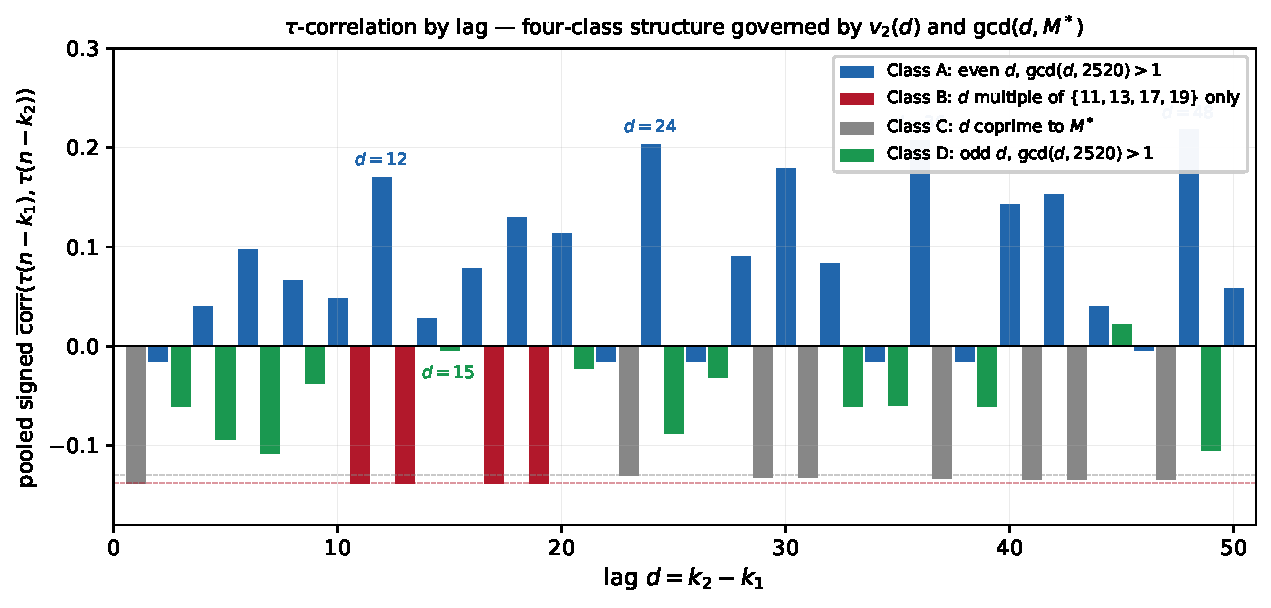
\includegraphics[width=0.85\linewidth]{figures/multipoint_tau_lag_profile.pdf}
\caption{Pooled signed correlation as a function of lag
$d \in [1, 50]$, color-coded by the four-class decomposition of
\cref{tab:correlation-decomposition}. Class A peaks (positive,
even $d$ with $\gcd(d, 2520) > 1$) appear at $d \in \{12, 24, 36, 48\}$
in this range. Class D destructive-interference cancellations
appear near $d = 15, 21, 45, 49$ (odd $d$ with $\gcd(d, 2520) > 1$).
Reference dashed lines mark the Class C background floor at
$-0.13$ and the Class B uniform value at $-0.138$.}
\label{fig:multipoint-tau-lag-profile}
\end{figure}

The mean off-diagonal $|\mathrm{corr}|$ over the full
$100 \times 100$ matrix is $0.0916$, with maximum $0.276$ at
$d = 60$. Independence would predict mean $|\mathrm{corr}| \ll 0.01$;
the observed pattern is the Bateman--Horn singular series visible
empirically through the framework reduction.

\subsubsection*{Per-class uniformity}

The four-class correlation pattern is itself \emph{class-uniform}.
Across all $41$ classes, the per-class mean off-diagonal
$|\mathrm{corr}|$ has mean $0.09163$ and standard deviation
$0.00028$ --- extraordinarily tight. The four sentinel classes
$\{858, 1716, 2431, 4862\}$ that admit a universal diagonal
mega-shift kill (\cref{sec:diagonal-megashift}) have mean
$|\mathrm{corr}| = 0.0914$ versus non-sentinel mean $0.0917$, a
difference of $-0.00025$, well within $1\sigma = 0.00028$.

The framework reduction therefore exhibits two \emph{independent}
empirical features:
\begin{itemize}[leftmargin=*]
\item a class-specific kernel structure (the diagonal mega-shift
  kill at $k_\Delta = 2520\, r$ for the sentinel residues, per
  \cref{sec:diagonal-megashift});
\item a class-uniform correlation pattern (the four-class lag
  decomposition above).
\end{itemize}
The conditional barrier theorem (\cref{thm:conditional-barrier})
predicts ``Schinzel-H survivors are non-uniformly distributed
according to local arithmetic structure''; the empirical correlation
matrix and the class-specific structural-kill identity provide two
independent quantitative anchors for that prediction, supporting
the conditional-barrier narrative without entailing closure.\footnote{An
apparent marginal outlier at $r = 13013$ in the original
$10^5$-sample run (max $\tauf = 10{,}368$, vs.\ median max $5{,}382$
across the $41$ classes) was investigated by an independent-seed
$10^6$-sample rerun: max $\tauf$ regressed to $6{,}480$, with mean
and median identical to the other classes. The original value was a
single Erd\H{o}s--Kac heavy-tail draw specific to the seed used in
the $10^5$-sample run, not a structural feature of the residue
class. Independently, the all-$41$ diagonal-B1 triage of
\cref{sec:branch-gluing-phaseB} returned SAT for $r = 13013$ at the
extended $600$\,s solver budget, in line with the other $40$
non-edge residues; the longer wall time reflects encoding-level
solver-difficulty variation rather than any structural property of
the residue. Both findings indicate $r = 13013$ is structurally
unremarkable.}

\subsection{The 40 non-principal residues}
\label{sec:empirical-nonprincipal}

The 40 non-principal residues in $\Ropen \setminus \{0\}$ have
\emph{not} been empirically verified at scale. The witness-search
infrastructure operates on every residue equally, and a few small
samples at non-principal residues have been collected, but no
non-principal residue has a documented empirical floor approaching
that of $r = 0$. We record this gap explicitly.

\begin{problem}[Empirical extension to non-principal residues]
\label{prob:non-principal-empirical}
For each $r \in \Ropen \setminus \{0\}$, establish a contiguous
empirical floor at $r$ comparable in scale to that of the principal
residue. Specifically, certify $N_r \ge 10^{20}$ for each such
$r$, with logged verifier output.
\end{problem}

The problem is finite-checkable but compute-intensive: at the
density of $\Ropen$ (one residue per $46189$ in unrestricted $\N$),
contiguous verification of any non-principal residue to $10^{20}$
requires $\sim 10^{16}$ candidate checks at the per-residue rate.
The principal-residue floor took several months of contiguous CPU
time on the project's infrastructure; an analogous campaign on each
of the 40 non-principal residues is correspondingly expensive.
\Cref{prob:non-principal-empirical} identifies this as the natural
empirical follow-up to the audit chain.

\subsection{Runtime, reproducibility, and audit}
\label{sec:empirical-runtime}

The contiguous principal-residue verifier was run on a single
high-throughput Hetzner CPX node over a multi-month campaign; the
high-shift sampler runs intermittently on the same infrastructure;
the 13-fold verifier is a one-shot Python script that ran in under
a minute per candidate. All three programs produce JSON logs
(\texttt{data/witness\_log.jsonl},
\texttt{data/sentinel\_log.jsonl},
\texttt{data/13fold\_log.jsonl}) recording every candidate examined
and the certifying shift $k$ for ruled-out candidates.

The verifier outputs are auditable in two senses:
\begin{itemize}[leftmargin=*]
\item \textbf{Per-candidate replay.} For any individual candidate
  in the log, the certifying shift $k$ and the divisor count
  $\tauf(n - k)$ can be recomputed independently in seconds; this
  is a single-candidate pen-and-paper check on a modest number.
\item \textbf{Coverage replay.} For the contiguous regime, the set
  of $n$ values checked is fully determined by the residue and the
  bound; an independent verifier can rerun any sub-range and
  compare logs. The non-contiguous regime is reproducible from the
  sampler's seed and the candidate-identification rules.
\end{itemize}

The empirical content is recorded as (C3) audit evidence in the
trust-chain summary of \cref{tab:trust-chain}. We do not promote
the empirical floor to a Lean-certified theorem in this paper:
formalization of an exhaustive numerical search of this scale is
not the appropriate locus of formal proof for a published bound.

\subsection{What the empirical floor licenses}
\label{sec:empirical-license}

We close with the strict logical content of the empirical content
of this section.

\emph{The empirical floor at $r = 0$ licenses:} a contiguous
no-counterexample claim at the principal residue up to $3.34
\times 10^{21}$, and consistency of the audit-chain barrier
picture with the predicted Bateman--Horn density at the two
13-fold witness points.

\emph{The empirical floor does not license:} any claim at $n >
3.34 \times 10^{21}$ at $r = 0$; any claim at any $n$ at the 40
non-principal residues; closure of any residue class; or any
upper or lower bound on the count of $\tauf$-barrier
counterexamples below $10^{22}$ in $\Ropen \setminus \{0\}$.

The barrier of this paper is the conjunction of the structural
reduction (\cref{sec:structural-reduction}), the finite-local audit
(\cref{sec:csp-audit}), and the analytic obstruction analysis
(\cref{sec:obstructions}); the empirical floor is a complementary
piece of evidence, not a closure.

% =============================================================================
% End of section 5
% =============================================================================
